\documentclass[10pt,letterpaper]{article}

\usepackage[margin=0.78in]{geometry}
\usepackage{microtype}
\usepackage{amsmath,amssymb}
\usepackage{booktabs}
\usepackage{tabularx}
\usepackage{graphicx}
\usepackage{enumitem}
\usepackage{xcolor}
\usepackage{url}
\usepackage[hidelinks]{hyperref}
\usepackage{caption}

\definecolor{paperblue}{HTML}{1F5A8A}
\definecolor{papergray}{HTML}{56616F}
\newcommand{\tool}[1]{\texttt{#1}}
\newcommand{\mape}{\mathrm{MAPE}}
\newcommand{\sm}{\mathrm{SM}}
\newcommand{\lone}{\mathrm{L1}}
\newcommand{\ltwo}{\mathrm{L2}}

\title{Evidence-Bounded Trace-to-Frontier Replay for Modern NVIDIA GPUs}
\author{Chengao Shi\\
Department of Electronic and Computer Engineering\\
Hong Kong University of Science and Technology\\
\texttt{author email omitted in technical review draft}}
\date{Technical review draft -- October 2026}

\begin{document}
\maketitle

\begin{abstract}
Detailed GPU simulation is valuable precisely where it is expensive: modern
kernels combine SIMT scheduling, sectored caches, asynchronous data movement,
tensor instructions, and long-latency memory service.  We present an
evidence-bounded trace-to-frontier replay stack that turns an instrumented
NVIDIA execution into a deterministic, architecture-parameterized replay
without treating profiler output as a replay input.  The stack joins dynamic
warp instructions, active and predicate masks, lane-level sectors, placement,
and launches with a static SASS-control sidecar; replays four-partition SM
issue and dependencies; connects sectored L1, shared L2, and a typed memory
service envelope; and emits issue, modeled-completion, observation, and
unmodeled-tail frontiers separately.  We evaluate the same contract over 286
successful RTX 3090 Ti/SM86 workload captures and 339 successful
RTX 5090/SM120 captures, covering 12,392 and 11,558 replayed launches.
On the current publication-safe metric subset, global-load sector error is
0.210\% (SM86) and 0.010\% (SM120); global-L1 lookup-miss error is 9.828\% and
6.094\%; L2 lookup-miss error is 0.000\% and 2.297\%; and active IPC error is
14.487\% and 9.455\%, respectively.  We report elapsed IPC below a relaxed 15\%
bar but do not claim sub-10\% closure.  Sequential full replay of the 356-root
SM86 campaign takes 509.05 s externally (344.819 s of successful-row driver
time), compared with 242.530 s for the corresponding non-NCU workload pass;
these are campaign-boundary measurements rather than an Accel-Sim speedup.
Metric families above the 15\% bar, including DRAM-read traffic and some
completion frontiers, remain explicit future work.  The contribution is the
replay contract and full-corpus evidence separation, not recovery of
proprietary RTL or a claim that trace-driven/event-driven simulation is new.
\end{abstract}

\section{Introduction}
\label{sec:intro}

GPU architects need to ask counterfactual questions about cache capacity,
latency, scheduling, and memory service before hardware exists.  A profiler
measures only the installed device, while an execution-driven simulator can
change the machine but pays the cost of reconstructing program behavior and
microarchitectural state.  A trace-driven simulator lies between these
extremes: it preserves a recorded dynamic path and spends modeling effort on
the proposed architecture.  The danger is that a trace can be mistaken for a
complete timing history, or that a favorable counter match can hide an
unmodeled state variable.

This paper presents a deterministic replay stack designed around that boundary.
The input is not an NCU table.  It is a dynamic NVBit-style trace and a static
SASS control sidecar.  The output is not one opaque ``cycle'' number.  It is a
set of named frontiers and counters whose causal ownership is explicit.  NCU
CSV files are joined only after replay, by capture/profile directory and launch
identity or ordered fallback, and are retained as independent observations.

Our goal is not to claim a first trace-driven or event-driven GPU simulator;
Accel-Sim, MGPUSim/Akita, NVArchSim, and modern GPU-core studies establish
those families~\cite{khairy2020accelsim,sun2019mgpusim,villa2021nvarchsim,huerta2025modern}.
Instead, we make four contributions:
\begin{enumerate}[leftmargin=1.35em,itemsep=2pt]
  \item a concrete dynamic-trace/static-SASS join that preserves warp, lane,
    sector, placement, and launch identities through issue and memory replay;
  \item a deterministic next-event implementation that keeps SM issue,
    sectored L1/L2 state, memory-service candidates, and wake-up causality in
    one inspectable path;
  \item an evidence contract that separates modeled state from profiler
    observation and separates issue, completion, observation, and typed-tail
    frontiers; and
  \item a complete-corpus evaluation on Ampere and Blackwell-class capture
    suites, with an accuracy table restricted to metrics that meet a declared
    15\% publication threshold and a runtime accounting that distinguishes
    workload, tracer, profiler, and simulator costs.
\end{enumerate}

The result is a practical architecture-study instrument: fast enough to replay
hundreds of real capture directories sequentially, detailed enough to expose
sector and readiness mechanisms, and conservative enough to leave unresolved
DRAM and completion semantics visible rather than fitting them away.

\section{Positioning and research boundary}
\label{sec:position}

\subsection{Established simulator families}

GPGPU-Sim established an execution-driven CUDA/GPU research platform, and
Accel-Sim made native NVIDIA instruction traces, correlation, and systematic
counter validation central to an open framework~\cite{khairy2020accelsim}.
MGPUSim/Akita and NVArchSim demonstrate event/protocol-driven and
variable-fidelity organization~\cite{sun2019mgpusim,villa2021nvarchsim}.
Huerta et al. characterize modern NVIDIA scheduler, control-word, register,
and dependency behavior~\cite{huerta2025modern}.  These works rule out
``trace-driven,'' ``event-driven,'' ``four-partition,'' and ``validated'' as
standalone novelty claims.

Recent systems occupy different abstraction points.  Sim-FA emphasizes
fine-grained asynchronous pipelines; GPU-Tile-Sim/GTSim represents optimized
kernels as warp-level tile graphs; PipeWeave combines analytical features and
learning; and TileSight provides a first-principles tile/system model.
Their goals and denominators differ from instruction-and-sector replay, so we
do not pool their errors with ours~\cite{simfa2026,gputilesim2026,pipeweave2026,tilesight2026}.
Dependency-enriched replay and causal validity are also established concerns;
Netrace and CausalSim show why a replay contract must name which dependencies
and external responses are preserved~\cite{netrace2010,causalsim2023}.

Our claim is therefore a systems integration claim: a trace-to-frontier
contract with explicit scope and full-corpus evidence.  We do not claim
proprietary cache hashes, MSHR counts, scheduler RTL, universal architecture
support, or a new general theory of trace sufficiency.

Figure~\ref{fig:sota-matrix} makes the comparison concrete.  Accel-Sim owns
the public native-SASS validation workflow; MGPUSim/Akita and NVArchSim own
event/protocol and industrial variable-fidelity precedents; Huerta et al. set a
modern NVIDIA core-fidelity reference; and Sim-FA, GPU-Tile-Sim/GTSim,
PipeWeave, and TileSight occupy asynchronous, tile, analytical, and learned
abstraction points.  Our differentiator is the intersection of native trace
identity, sector-aware causal replay, separated frontier semantics,
post-replay NCU joins, and complete 286/339-root evidence.  The matrix is
qualitative and deliberately does not sum heterogeneous capabilities into a
single score.

\begin{figure}[t]
  \centering
  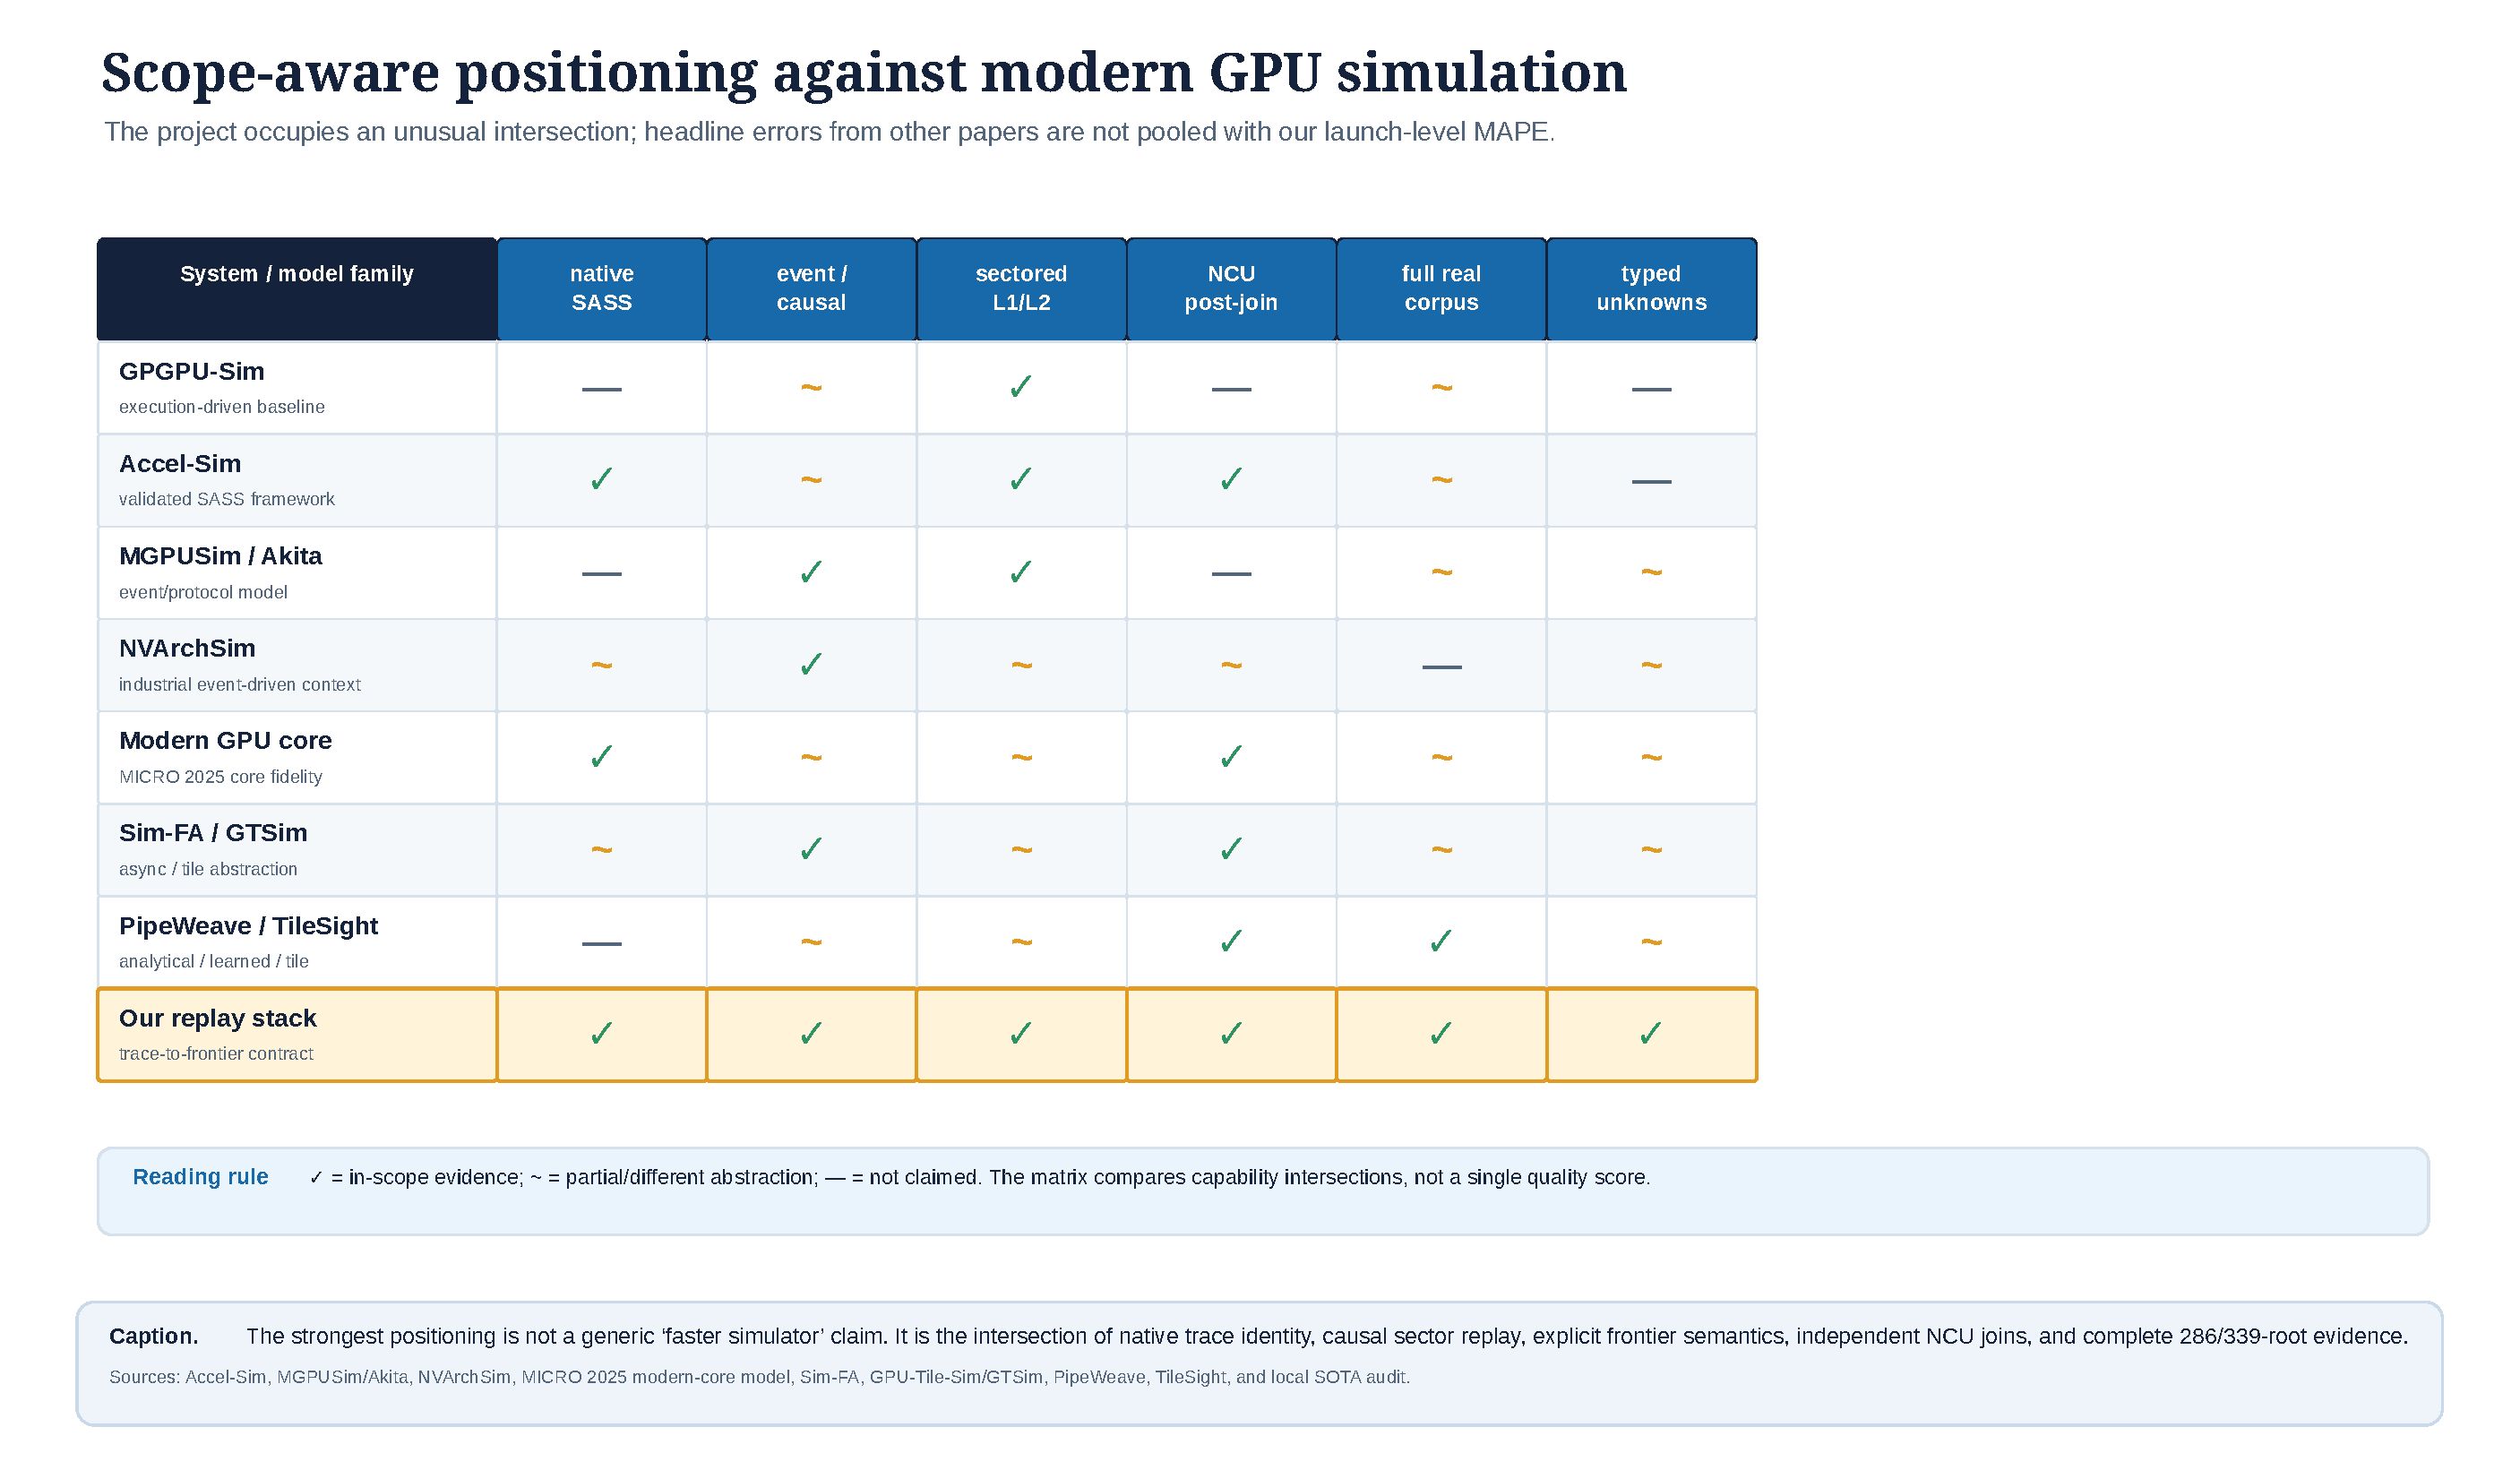
\includegraphics[width=\linewidth]{figures/sota_matrix.pdf}
  \caption{Scope-aware positioning against modern GPU simulation.  A checkmark
  denotes in-scope evidence, a tilde denotes partial or different abstraction,
  and a dash denotes a capability not claimed.  This is a capability
  intersection, not a scalar ranking of unrelated papers.}
  \label{fig:sota-matrix}
\end{figure}

The contemporary reported numbers sharpen the comparison but are not a pooled
leaderboard: the MICRO 2025 modern-core model reports 13.45\% mean MAPE;
Sim-FA reports 5.7\% MAPE for its H800 FlashAttention-3 study;
GPU-Tile-Sim reports 1.22--8.71\% on its A100/H100 tile workloads;
PipeWeave reports 6.1\% average kernel error and 8.5\% end-to-end inference
error; and TileSight reports 12.35\% pooled single-GPU MAPE and 13.52\%
serving weighted MAPE.  LPGSim reports 21.4--23.3\% cycle error across its
V100/A100/RTX3090 study and a 9.97$\times$ single-thread Accel-Sim speedup.
These values use different devices, workloads, abstractions, and denominators;
our paper therefore compares capability and scope, then reports our own
launch-level MAPE separately.

\begin{table}[t]
  \centering
  \caption{Reported contemporary SOTA results from the local literature audit.
  The values are context, not a cross-paper leaderboard; our launch-level
  metrics are reported separately in Table~\ref{tab:accuracy}.}
  \label{tab:sota-reported}
  \small
  \begin{tabularx}{\linewidth}{@{}p{2.2cm}p{3.0cm}p{3.0cm}X@{}}
    \toprule
    System & Abstraction / target & Reported result & Why it is not pooled here\\
    \midrule
    Modern GPU core & SASS/core, modern NVIDIA & 13.45\% mean MAPE & Different core model and cohort\\
    Sim-FA & Hopper async pipeline & 5.7\% MAPE & H800 FA3/TMA scope\\
    GPU-Tile-Sim & Warp-level tiles & 1.22--8.71\% MAPE & A100/H100 tile workloads\\
    PipeWeave & Analytical + learned & 6.1\% kernel; 8.5\% end-to-end & Prediction, not causal replay\\
    TileSight & First-principles tiles & 12.35\% single-GPU; 13.52\% serving & Tile/network abstraction\\
    LPGSim & Compressed SASS replay & 21.4--23.3\% cycle error; 9.97$\times$ Accel-Sim & Relaxed/local-clock policy\\
    \bottomrule
  \end{tabularx}
\end{table}

\section{Replay contract}
\label{sec:contract}

\subsection{Inputs and independent authority}

For each capture directory, the replay consumes:
\begin{itemize}[leftmargin=1.35em,itemsep=2pt]
  \item dynamic records containing PC, warp/block/SM identity, active and
    predicate masks, per-lane memory addresses, launch geometry, and opcode
    observations;
  \item a static SASS sidecar containing stall/yield bits, read/write barriers,
    wait masks, reuse information, and decoded memory forms; and
  \item an architecture card containing cache geometry, latencies, service
    assumptions, and typed unknowns.
\end{itemize}

The NCU profile is a post-replay authority.  The comparator first tries exact
capture/profile and launch identity; if compiler-generated kernel names differ,
it uses the stable capture directory and launch order.  A missing target row is
unmatched, not zero error.  Scope warnings remain in raw/all-row accounting and
are also reported in the secondary like-for-like view.

\begin{figure}[t]
  \centering
  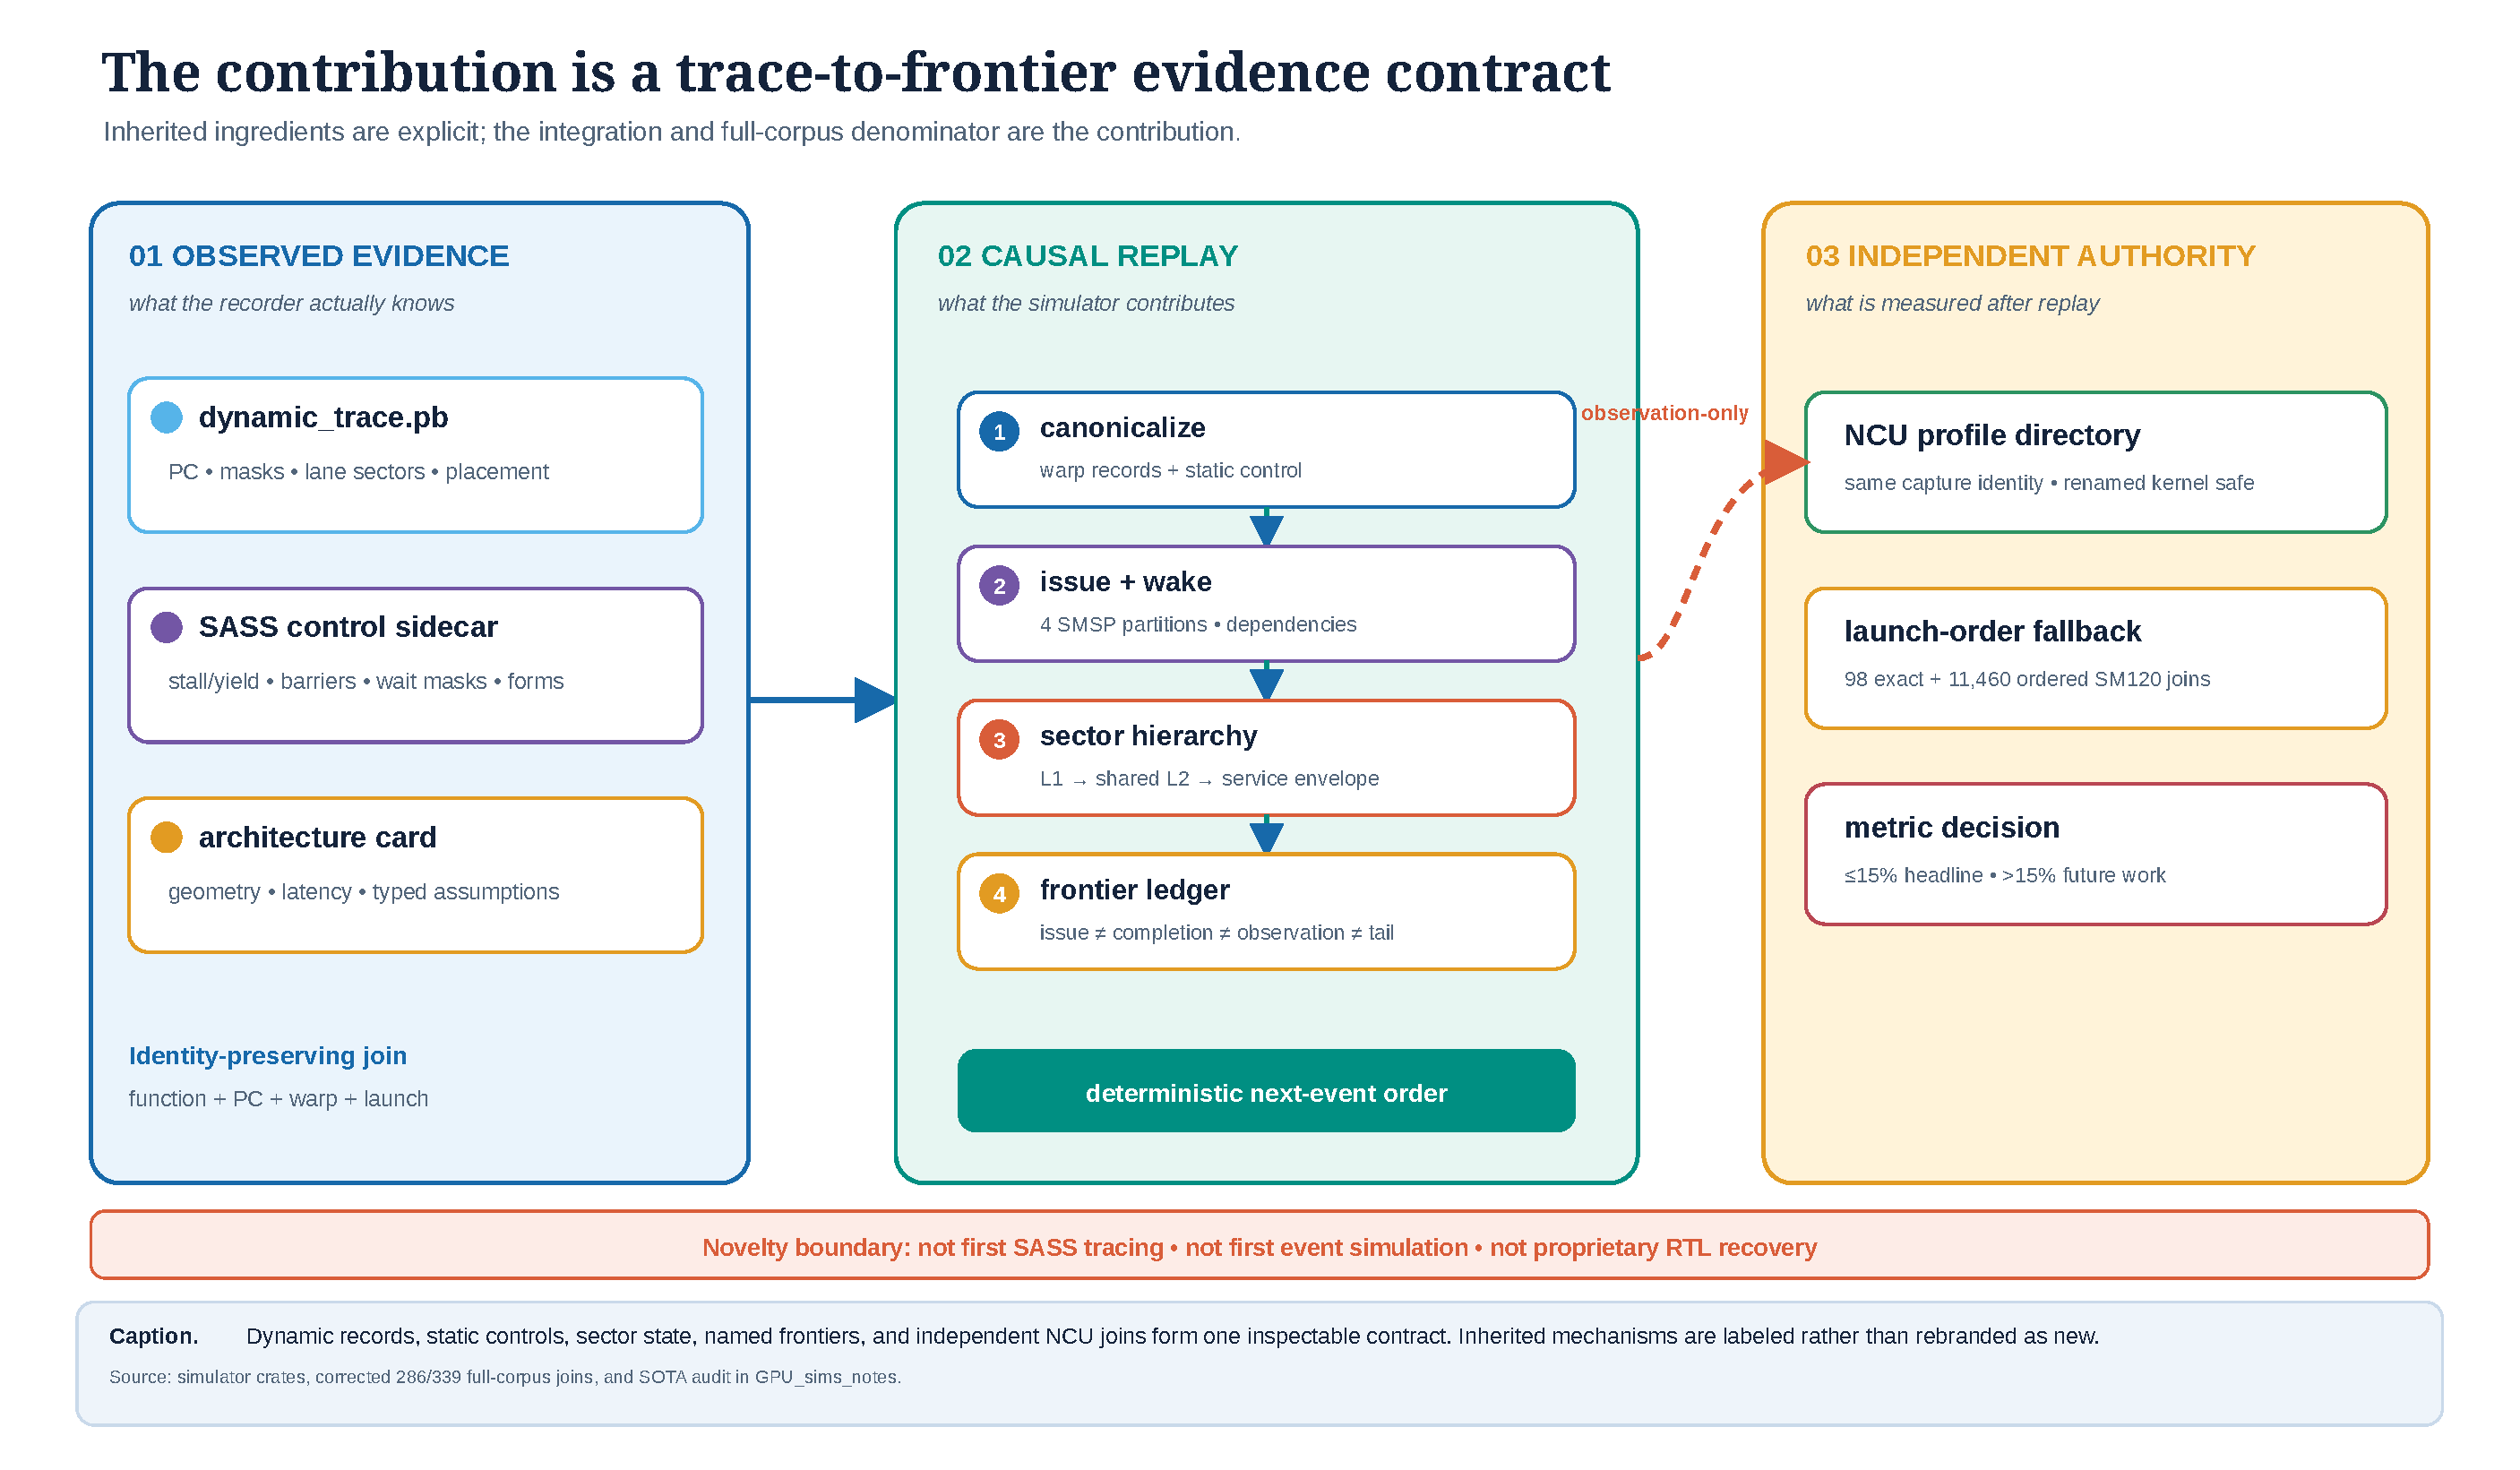
\includegraphics[width=\linewidth]{figures/novelty_stack.pdf}
  \caption{The contribution is a trace-to-frontier evidence contract.  The
    left panel shows what the recorder knows, the middle panel shows the causal
    replay integration, and the right panel shows the independent NCU authority
    and launch-scope decision.  The bottom boundary states what is inherited
    rather than claimed as new.}
  \label{fig:novelty-stack}
\end{figure}

\subsection{State and frontiers}

The replay maintains separate state for four SMSP issue partitions, per-warp
dependencies and barriers, sectored L1 lines and outstanding fills, shared-L2
lines and source lanes, and an aggregate memory-service envelope.  A binary
heap orders events by cycle and insertion sequence; idle intervals are skipped
without removing causal events.

We expose four frontiers:
\begin{enumerate}[leftmargin=1.35em,itemsep=2pt]
  \item the last-issue/issue frontier, which identifies the modeled SM work;
  \item the modeled completion frontier, which includes declared response and
    barrier consequences;
  \item the observation frontier, which describes how an NCU-shaped endpoint
    is projected from replay state; and
  \item typed tails for dirty writeback, coherence, asynchronous visibility,
    and engine completion that the trace does not establish.
\end{enumerate}

This separation prevents a terminal dirty line or an unobserved asynchronous
engine acknowledgement from silently becoming a kernel-cycle claim.

\section{SIMT execution and multi-threading strategy}
\label{sec:simt}

CPU simulation commonly represents each software thread as an independently
scheduled instruction stream.  Applying that strategy literally to a GPU would
create up to 32 host actors per warp, multiply event traffic, and still fail to
represent the GPU's lockstep lane semantics.  GPU SIMT is hierarchical:
threads are grouped into warps, a warp issues one instruction for its active
lanes, and multiple resident warps interleave when one warp is stalled on a
dependency, barrier, cache miss, or asynchronous operation.

There are three useful modeling choices:
\begin{enumerate}[leftmargin=1.35em,itemsep=2pt]
  \item \textbf{Functional per-thread execution} re-executes lane control flow
    and values.  It can respond to counterfactual timing, but has high host
    cost and requires a complete functional ISA, memory model, and race
    semantics.
  \item \textbf{Warp-level trace replay} stores one dynamic stream per warp,
    retains active/predicate masks and lane addresses, and schedules warps as
    the hardware does.  It is much cheaper and preserves observed coalescing,
    divergence, and placement, but cannot regenerate a path that a target
    intervention would change.
  \item \textbf{Tile/analytical or learned models} compress many instructions
    into tile actions or statistical features.  They are attractive for
    throughput and broad design sweeps, but can lose per-lane sector, barrier,
    and source-qualified cache detail.
\end{enumerate}

Our native SM86/SM120 path uses the second choice.  `sim-sm' is one resumable
host actor per SM.  Each physical warp slot maps to an SMSP by
`warp\_slot mod 4`; each SMSP selects at most one ready warp per issue cycle.
The scheduler keeps the held warp while it remains ready, drops the hold on a
compiler yield, and otherwise switches to the youngest ready warp.  A traced
instruction advances exactly one warp stream; its lane mask and sector arena
drive memory coalescing, while barriers, dependency waits, residency, and
responses determine when that warp can issue again.  CTA admission models
resident-warp/shared-memory limits and frees resources when a block finishes.

This is not a claim that the host runtime is a proprietary SM scheduler.  It is
an explicit effective model whose tradeoff is auditable: lane evidence remains
available to L1/L2, but the simulator does not pay for 32 independent host
threads per warp.  The contribution is the identity-preserving connection
between SIMT masks, SMSP interleaving, sector state, and named frontiers; the
individual ingredients have substantial prior art.

\begin{figure}[t]
  \centering
  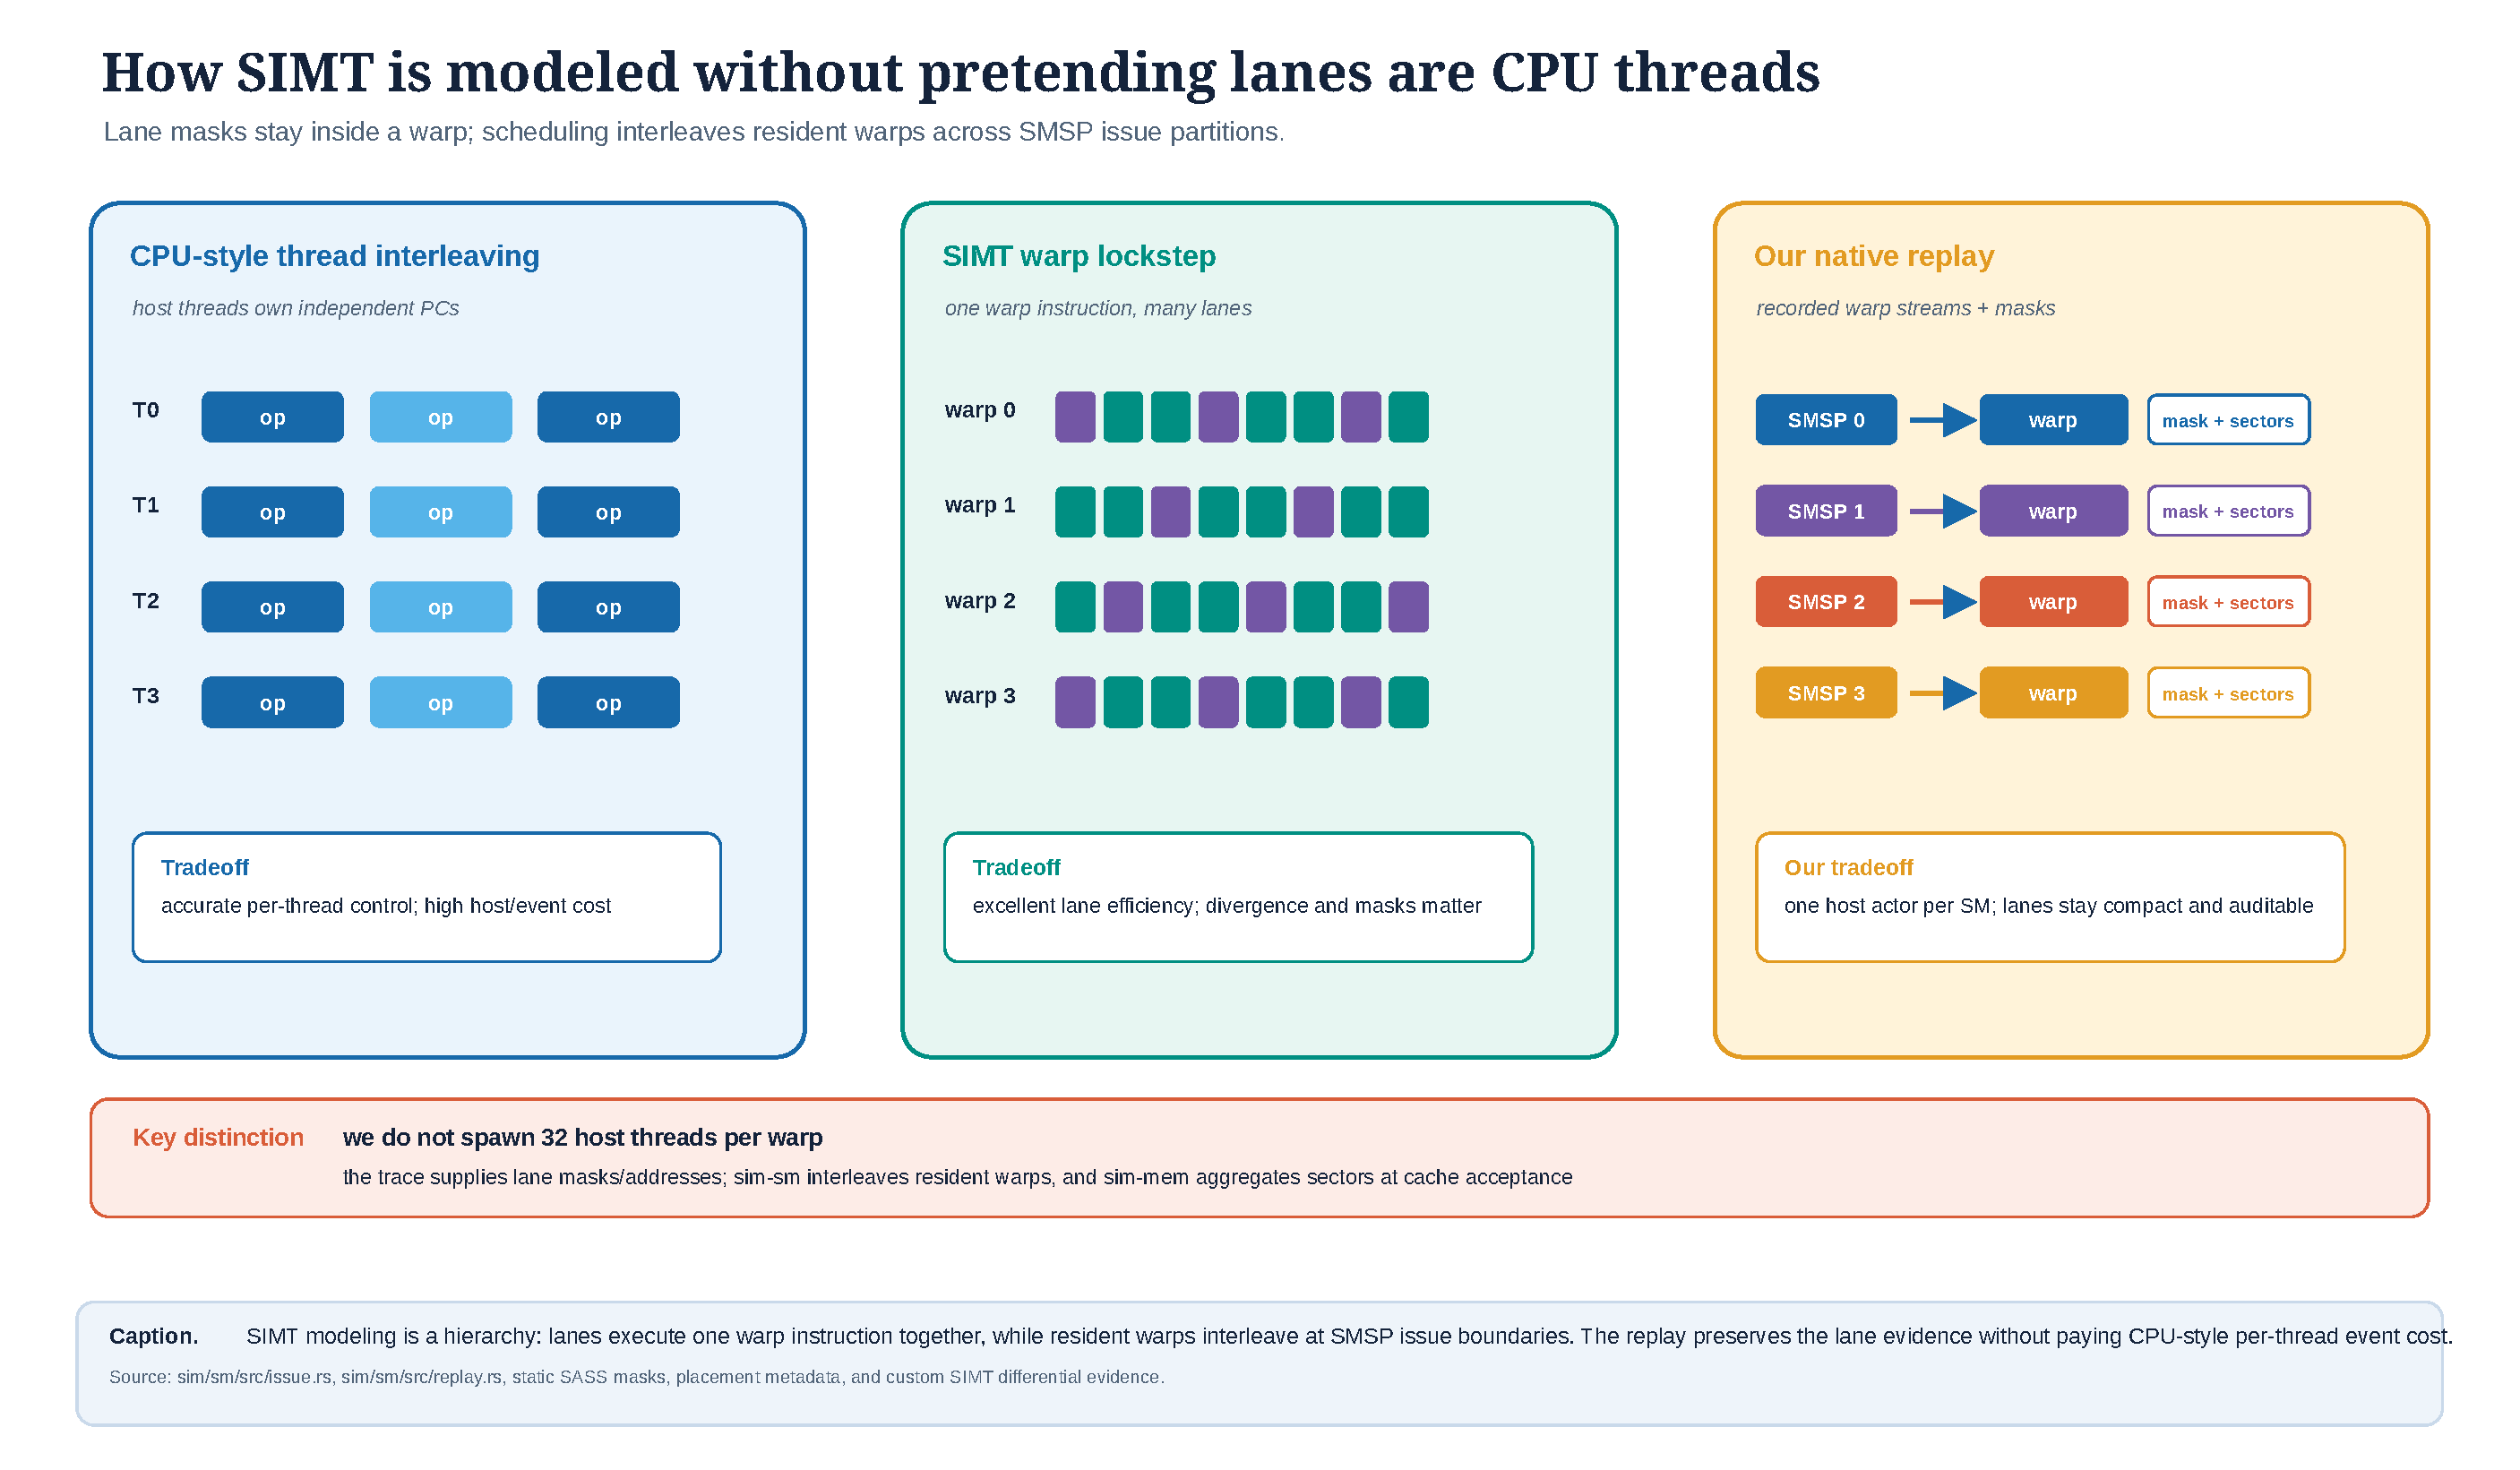
\includegraphics[width=\linewidth]{figures/simt_interleaving.pdf}
  \caption{SIMT execution strategy and tradeoffs.  CPU-style thread
  interleaving, warp lockstep, and the replay's one-host-actor-per-SM model are
  separated.  Lane masks stay inside a warp; resident warps interleave at SMSP
  issue boundaries.}
  \label{fig:simt-interleaving}
\end{figure}

\begin{figure}[t]
  \centering
  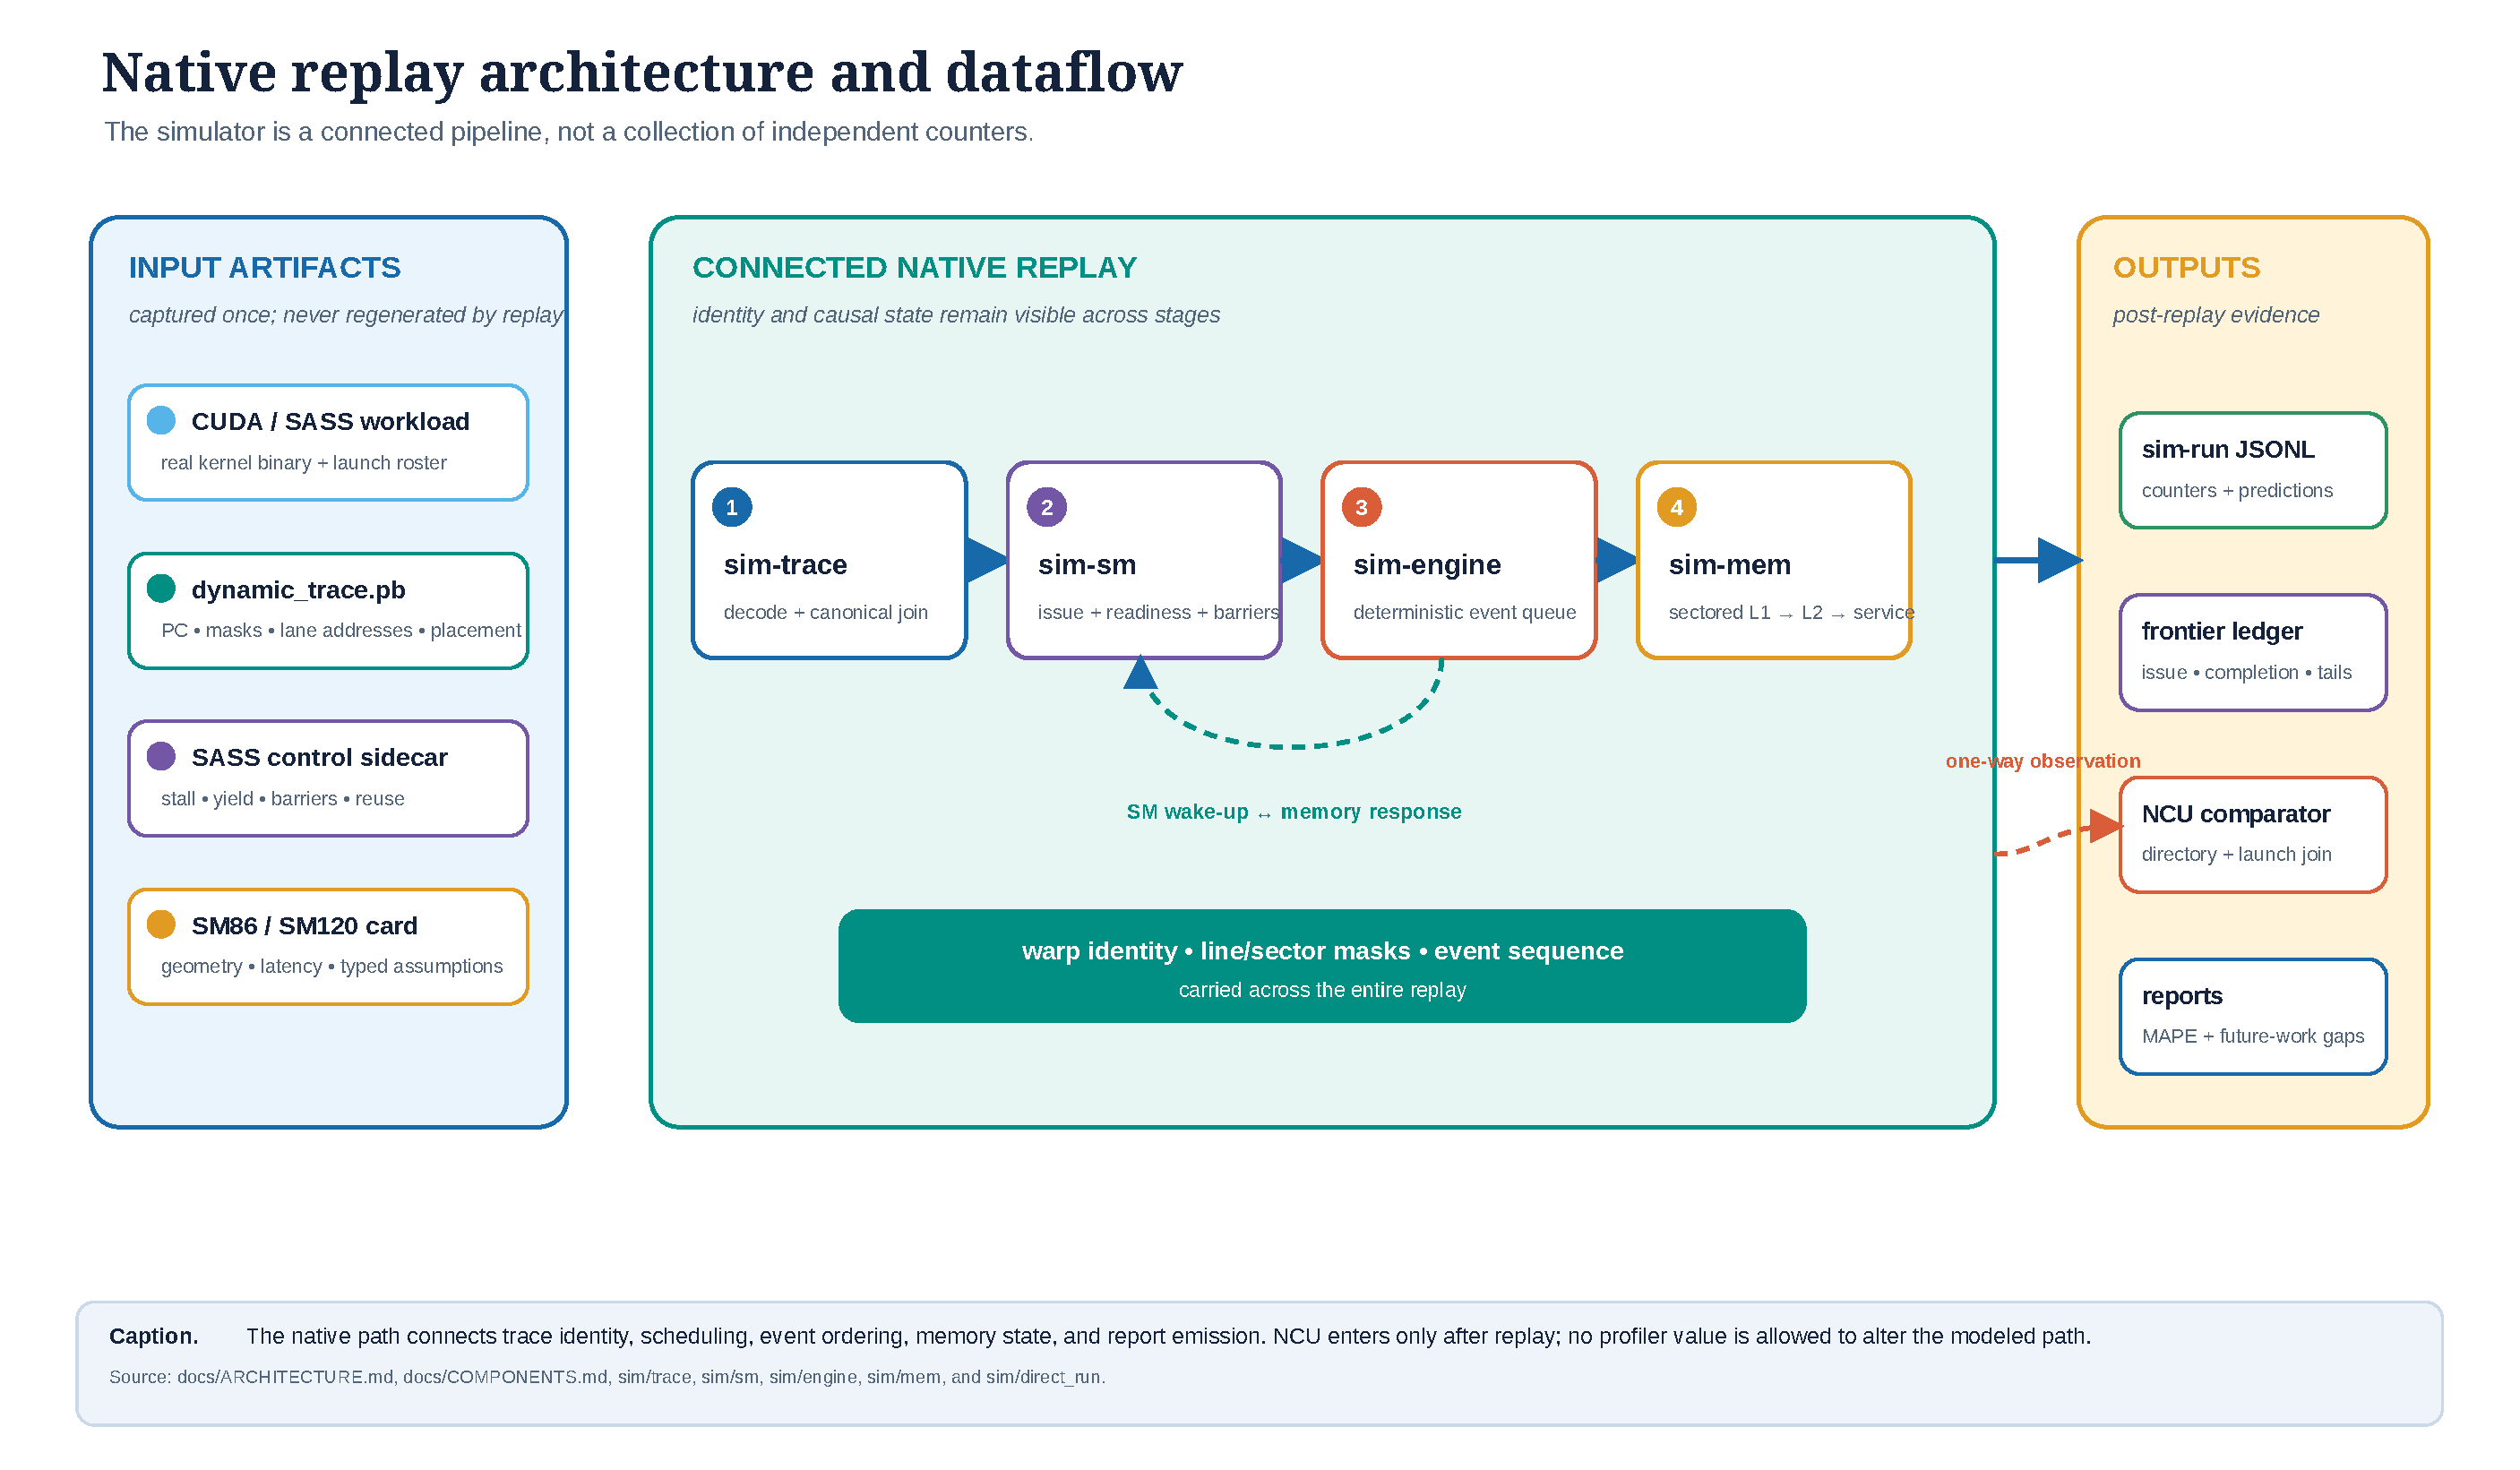
\includegraphics[width=\linewidth]{figures/architecture_pipeline.pdf}
  \caption{Native replay architecture and dataflow.  Concrete workload,
  trace, sidecar, and card artifacts flow through `sim-trace', `sim-sm',
  `sim-engine', and `sim-mem' before `sim-run' emits JSONL counters and
  frontiers.  NCU is a one-way post-replay comparator.}
  \label{fig:architecture-pipeline}
\end{figure}

\begin{figure}[t]
  \centering
  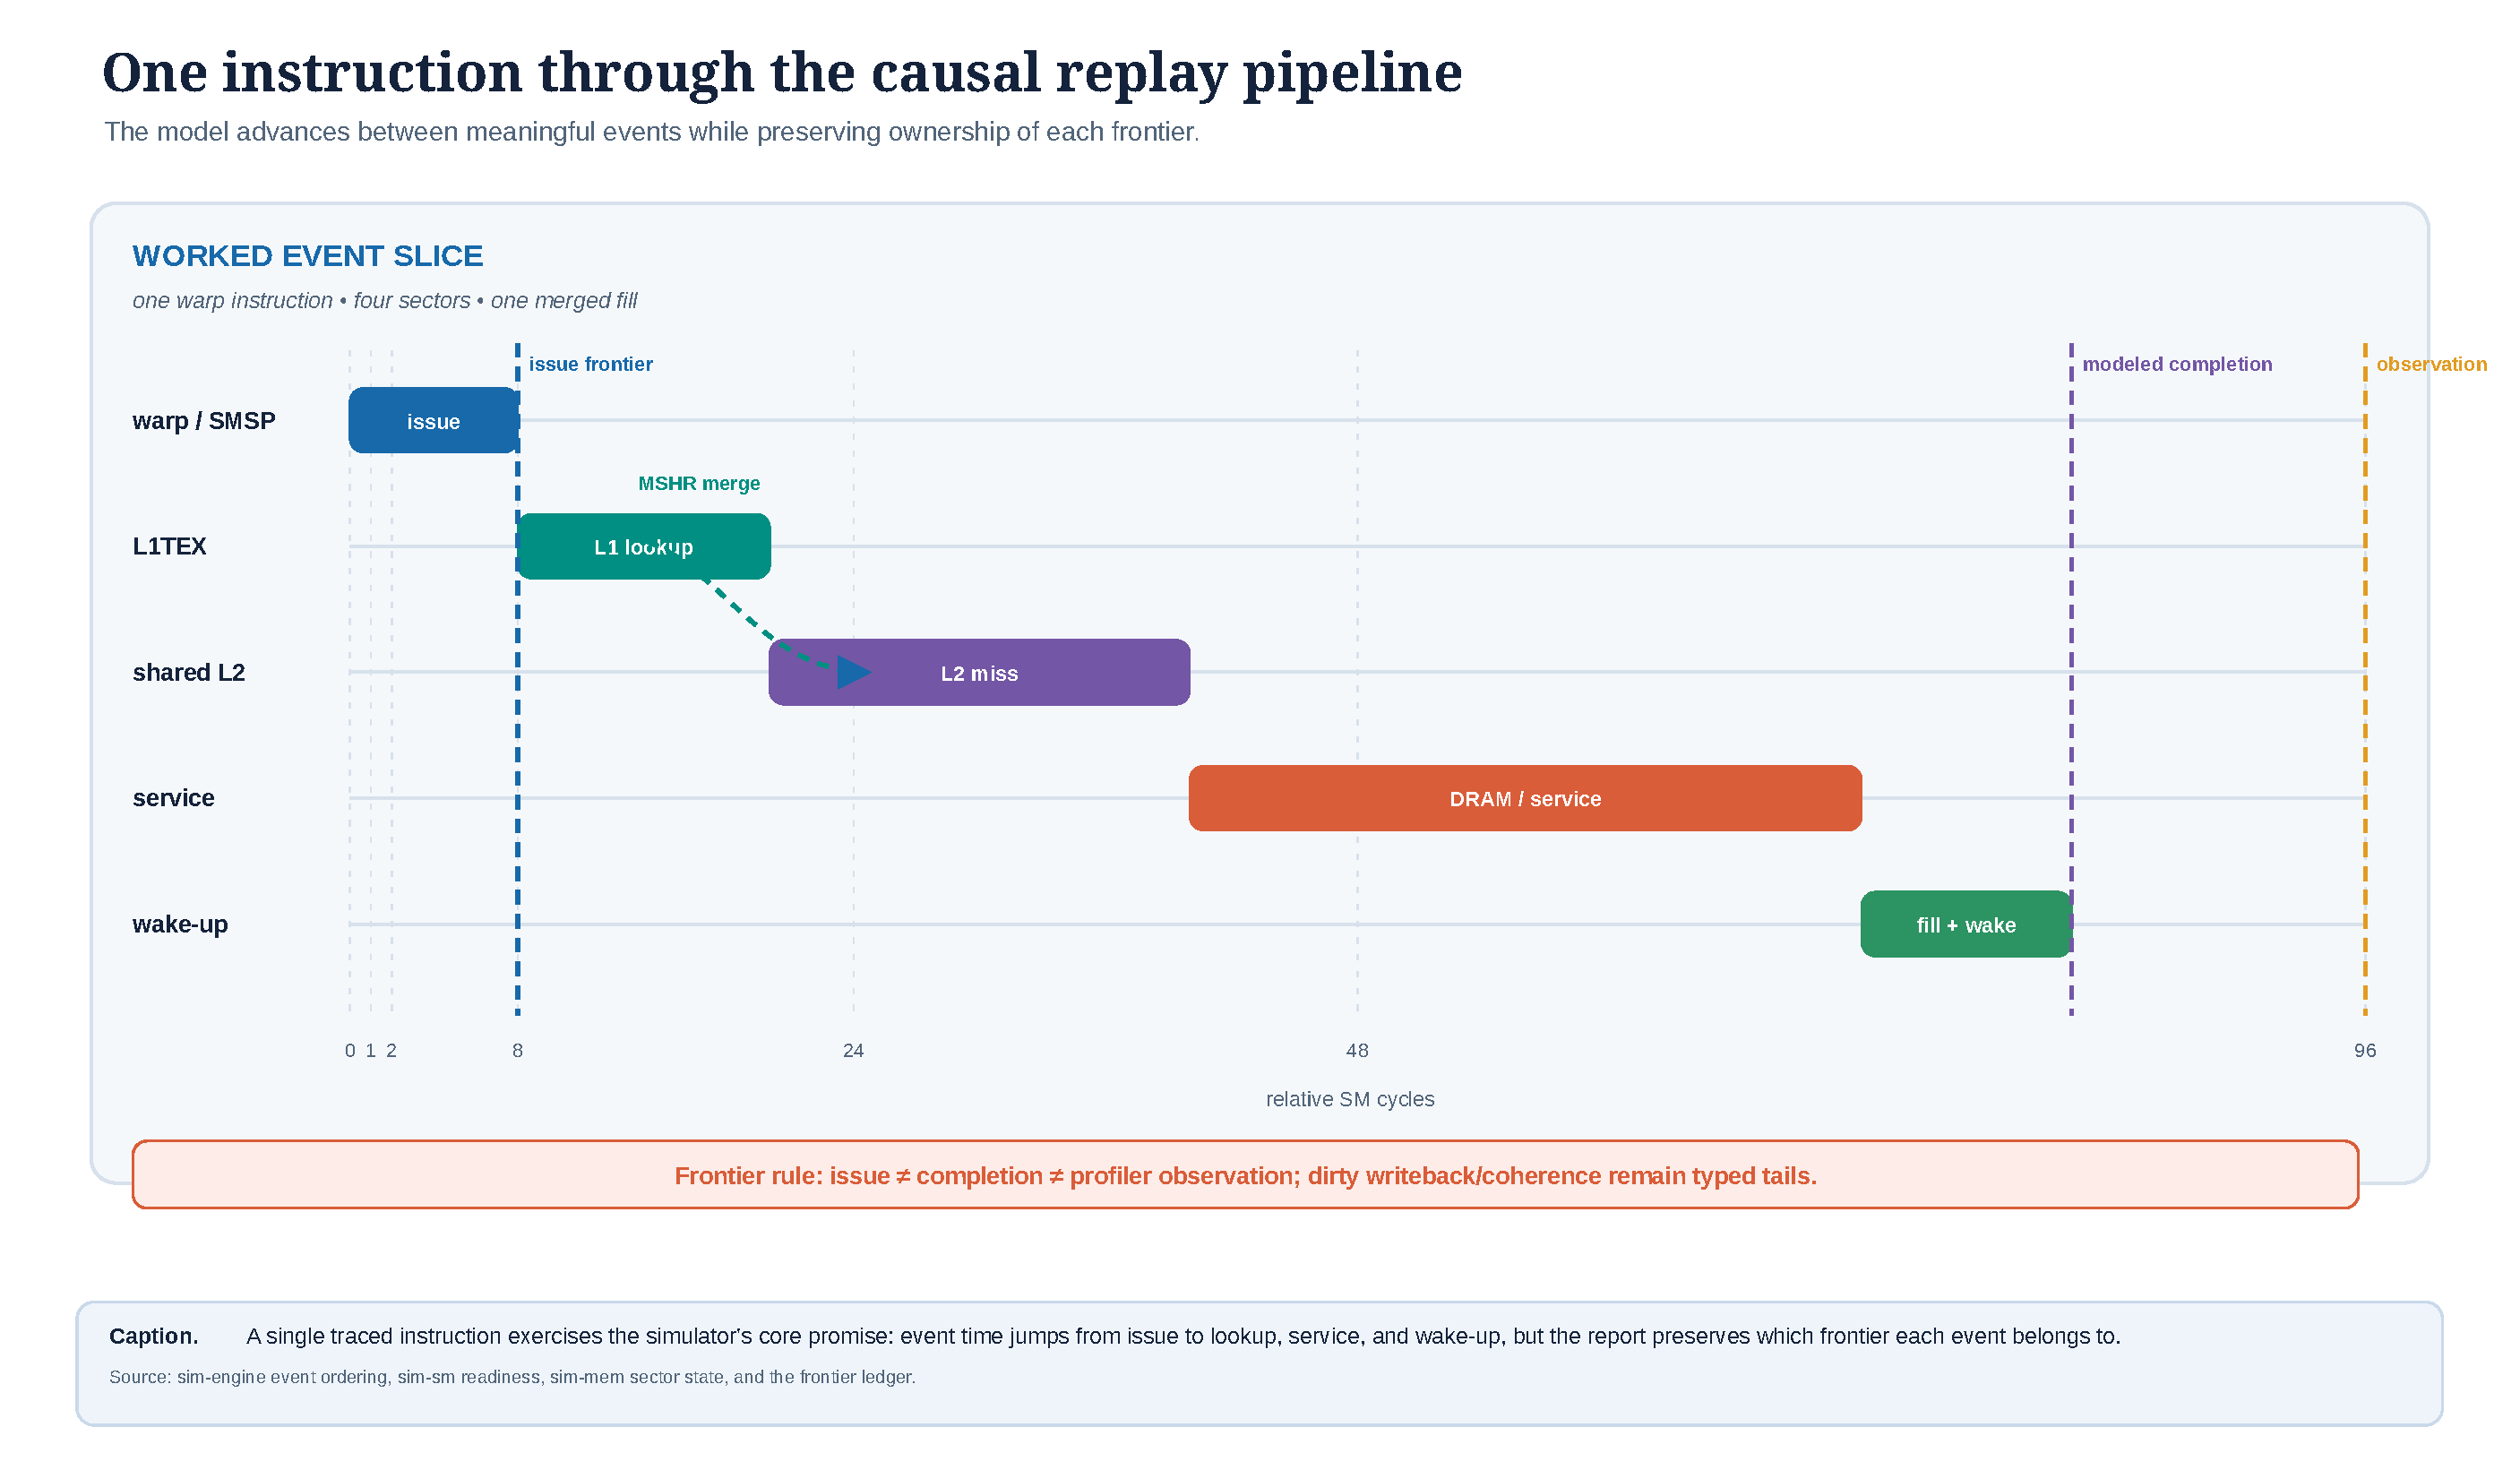
\includegraphics[width=\linewidth]{figures/causal_timeline.pdf}
  \caption{One instruction through the causal replay pipeline.  The worked
  slice separates issue, L1 lookup, shared-L2 miss, service, fill/wake-up, and
  the three report frontiers; the MSHR merge is explicit rather than hidden in
  a scalar latency.}
  \label{fig:causal-timeline}
\end{figure}

\section{Implementation}
\label{sec:implementation}

\subsection{Trace reconstruction and issue}

The trace reader groups operand observations into one dynamic warp instruction,
canonicalizes active/predicate masks, and retains per-lane sectors.  The static
join is keyed by function identity and PC.  The SM model uses four scheduling
partitions, compiler-guided stall/yield controls, register/dependency horizons,
barrier generations, modeled residency, and response-driven warp wake-up.
Every admitted record increments one instruction counter; the replay asserts
that the number of issued records equals the records supplied by the capture.
This is a replay-integrity invariant, not an independent control-flow
prediction.

\subsection{Sector-aware memory hierarchy}

Lines contain four 32-byte sectors.  L1 tracks valid sectors, pending fills,
line allocations, and operation-qualified observers.  L2 is shared and
sectored; reads, stores, atomics, reductions, and asynchronous payload shadows
retain distinct source/operation counters.  The memory-service layer prices
declared demand with a typed aggregate envelope.  A prototype DRAM card is
enabled for the SM120 full replay, but its bandwidth values are explicitly
marked unvalidated; the conservative disabled run is retained.

\subsection{Metric projections}

The simulator emits instruction cardinalities, global load/store sectors,
operation-qualified L2 sectors and lookup splits, shared-memory wavefronts,
cache-rate projections, IPC projections, and GPC/SM frontier observations.
Each prediction carries its source and semantics.  For example, a TMA payload
sector count is labeled conditional demand rather than an achieved DRAM
acknowledgement, and an IPC projection is labeled model-relative rather than a
silicon issue-width measurement.

\section{Experimental method}
\label{sec:method}

\subsection{Corpora and replay configuration}

The SM86 corpus contains 356 capture roots: 286 successful workload roots, 62
typed mixed-code controls, and 8 replay/input failures.  The full replay covers
12,392 launches.  The locked reference point is an RTX 3090 Ti at 1350 MHz SM
and 10501 MHz memory.  The SM120 corpus contains 339 successful roots and
11,558 launches from the RTX 5090 capture suite.  The SM120 full replay uses
the integrated effective L1/L2 lane; DRAM-disabled and prototype-carded runs
are both retained.

All generated replay JSONL artifacts are compressed.  Full replay precedes any
fast complementary lane.  NCU values are never consumed by the simulator or
used to select a card parameter.

\subsection{Join and scoring rules}

For SM86, the latest accepted report has 107 exact identity joins; the
publication table uses the metric-specific compatible subset (normally 104--
107 rows).  For SM120, compiler-generated names differ more often.  We join
within the same capture/profile directory and launch order after exact identity;
the enabled full artifact yields 98 exact rows and 11,460 ordered-fallback rows,
covering all 11,558 replay launches.  This is a directory-scoped
correspondence, not a string-match assumption.

The two profile campaigns intentionally have different launch scopes.  The
SM86 NCU wrapper used `--launch-count 1`, so each of its 356 profile directories
contains one profiled launch; the 104--107-row metric counts therefore describe
all finite target rows present in that one-launch-per-directory campaign, not
all 12,392 replay launches.  The SM120 wrapper profiles all matching launches,
and the corrected 339-directory reduction covers every 11,558 replay launches.
This distinction is retained in the denominator rather than hidden by pooling
capture counts and launch counts.

For a target $y$ and prediction $\hat y$, the row error is
\[
  e(y,\hat y) = \frac{|\hat y-y|}{|y|},
\]
with zero-target rows handled by exact-zero rules.  We report mean APE only
for finite nonzero target opportunities and retain raw/all-row scope warnings
separately.  The paper headline includes metrics at or below 15\%; important
families above that threshold are future work rather than favorable numbers.

\section{Results}
\label{sec:results}

\subsection{Architectural metric accuracy}

Table~\ref{tab:accuracy} reports the publication-safe subset.  SM86 values are
from the H116 full-first report; SM120 values are from the enabled full-only
directory/ordered-fallback reduction.  Counts are launch-level comparison
opportunities, not the number of capture roots.

\begin{table}[t]
  \centering
  \caption{Mean absolute percentage error on complete-corpus replay joins.
  Only metrics at or below the declared 15\% publication bar are headline
  results.  ``Active'' and ``elapsed'' IPC use the simulator's model-relative
  projection semantics.}
  \label{tab:accuracy}
  \small
  \begin{tabular}{@{}lrrr rrr@{}}
    \toprule
    & \multicolumn{3}{c}{SM86 / RTX 3090 Ti} & \multicolumn{3}{c}{SM120 / RTX 5090}\\
    Metric & MAPE & Rows & Status & MAPE & Rows & Status\\
    \midrule
    Global-load sectors & 0.210\% & 106 & report & 0.010\% & 11,558 & report\\
    Global-store sectors & 0.000\% & 107 & report & 0.474\% & 11,558 & report\\
    Global L1 lookup misses & 9.828\% & 106 & report & 6.094\% & 11,558 & report\\
    L2 TEX lookup misses & 0.000\% & 104 & report & 2.297\% & 11,558 & report\\
    L2 read lookup misses & 0.000\% & 104 & report & 0.031\% & 11,556 & report\\
    Shared-load wavefronts & 5.623\% & 107 & report & 7.250\% & 11,558 & report\\
    Shared-store wavefronts & 2.418\% & 107 & report & 0.084\% & 11,558 & report\\
    Active IPC & 14.487\% & 107 & <15\% & 9.455\% & 11,558 & <10\%\\
    Elapsed IPC & 12.307\% & 107 & <15\% & 13.602\% & 11,558 & <15\%\\
    \bottomrule
  \end{tabular}
\end{table}

The table demonstrates two properties.  First, sector denominators and
operation-qualified lookup-miss surfaces are stable across substantially
different targets and workload families.  Second, the timing projections are
useful but not closed at the preferred 10\% threshold on both architectures.
We intentionally do not headline DRAM-read traffic, aggregate L2 lookup hits,
unified hit rates, or GPC/SM completion families whose current residuals or
scope contracts do not meet the declared bar.  They remain in the compressed
metric reports and in the future-work section.

\begin{figure}[t]
  \centering
  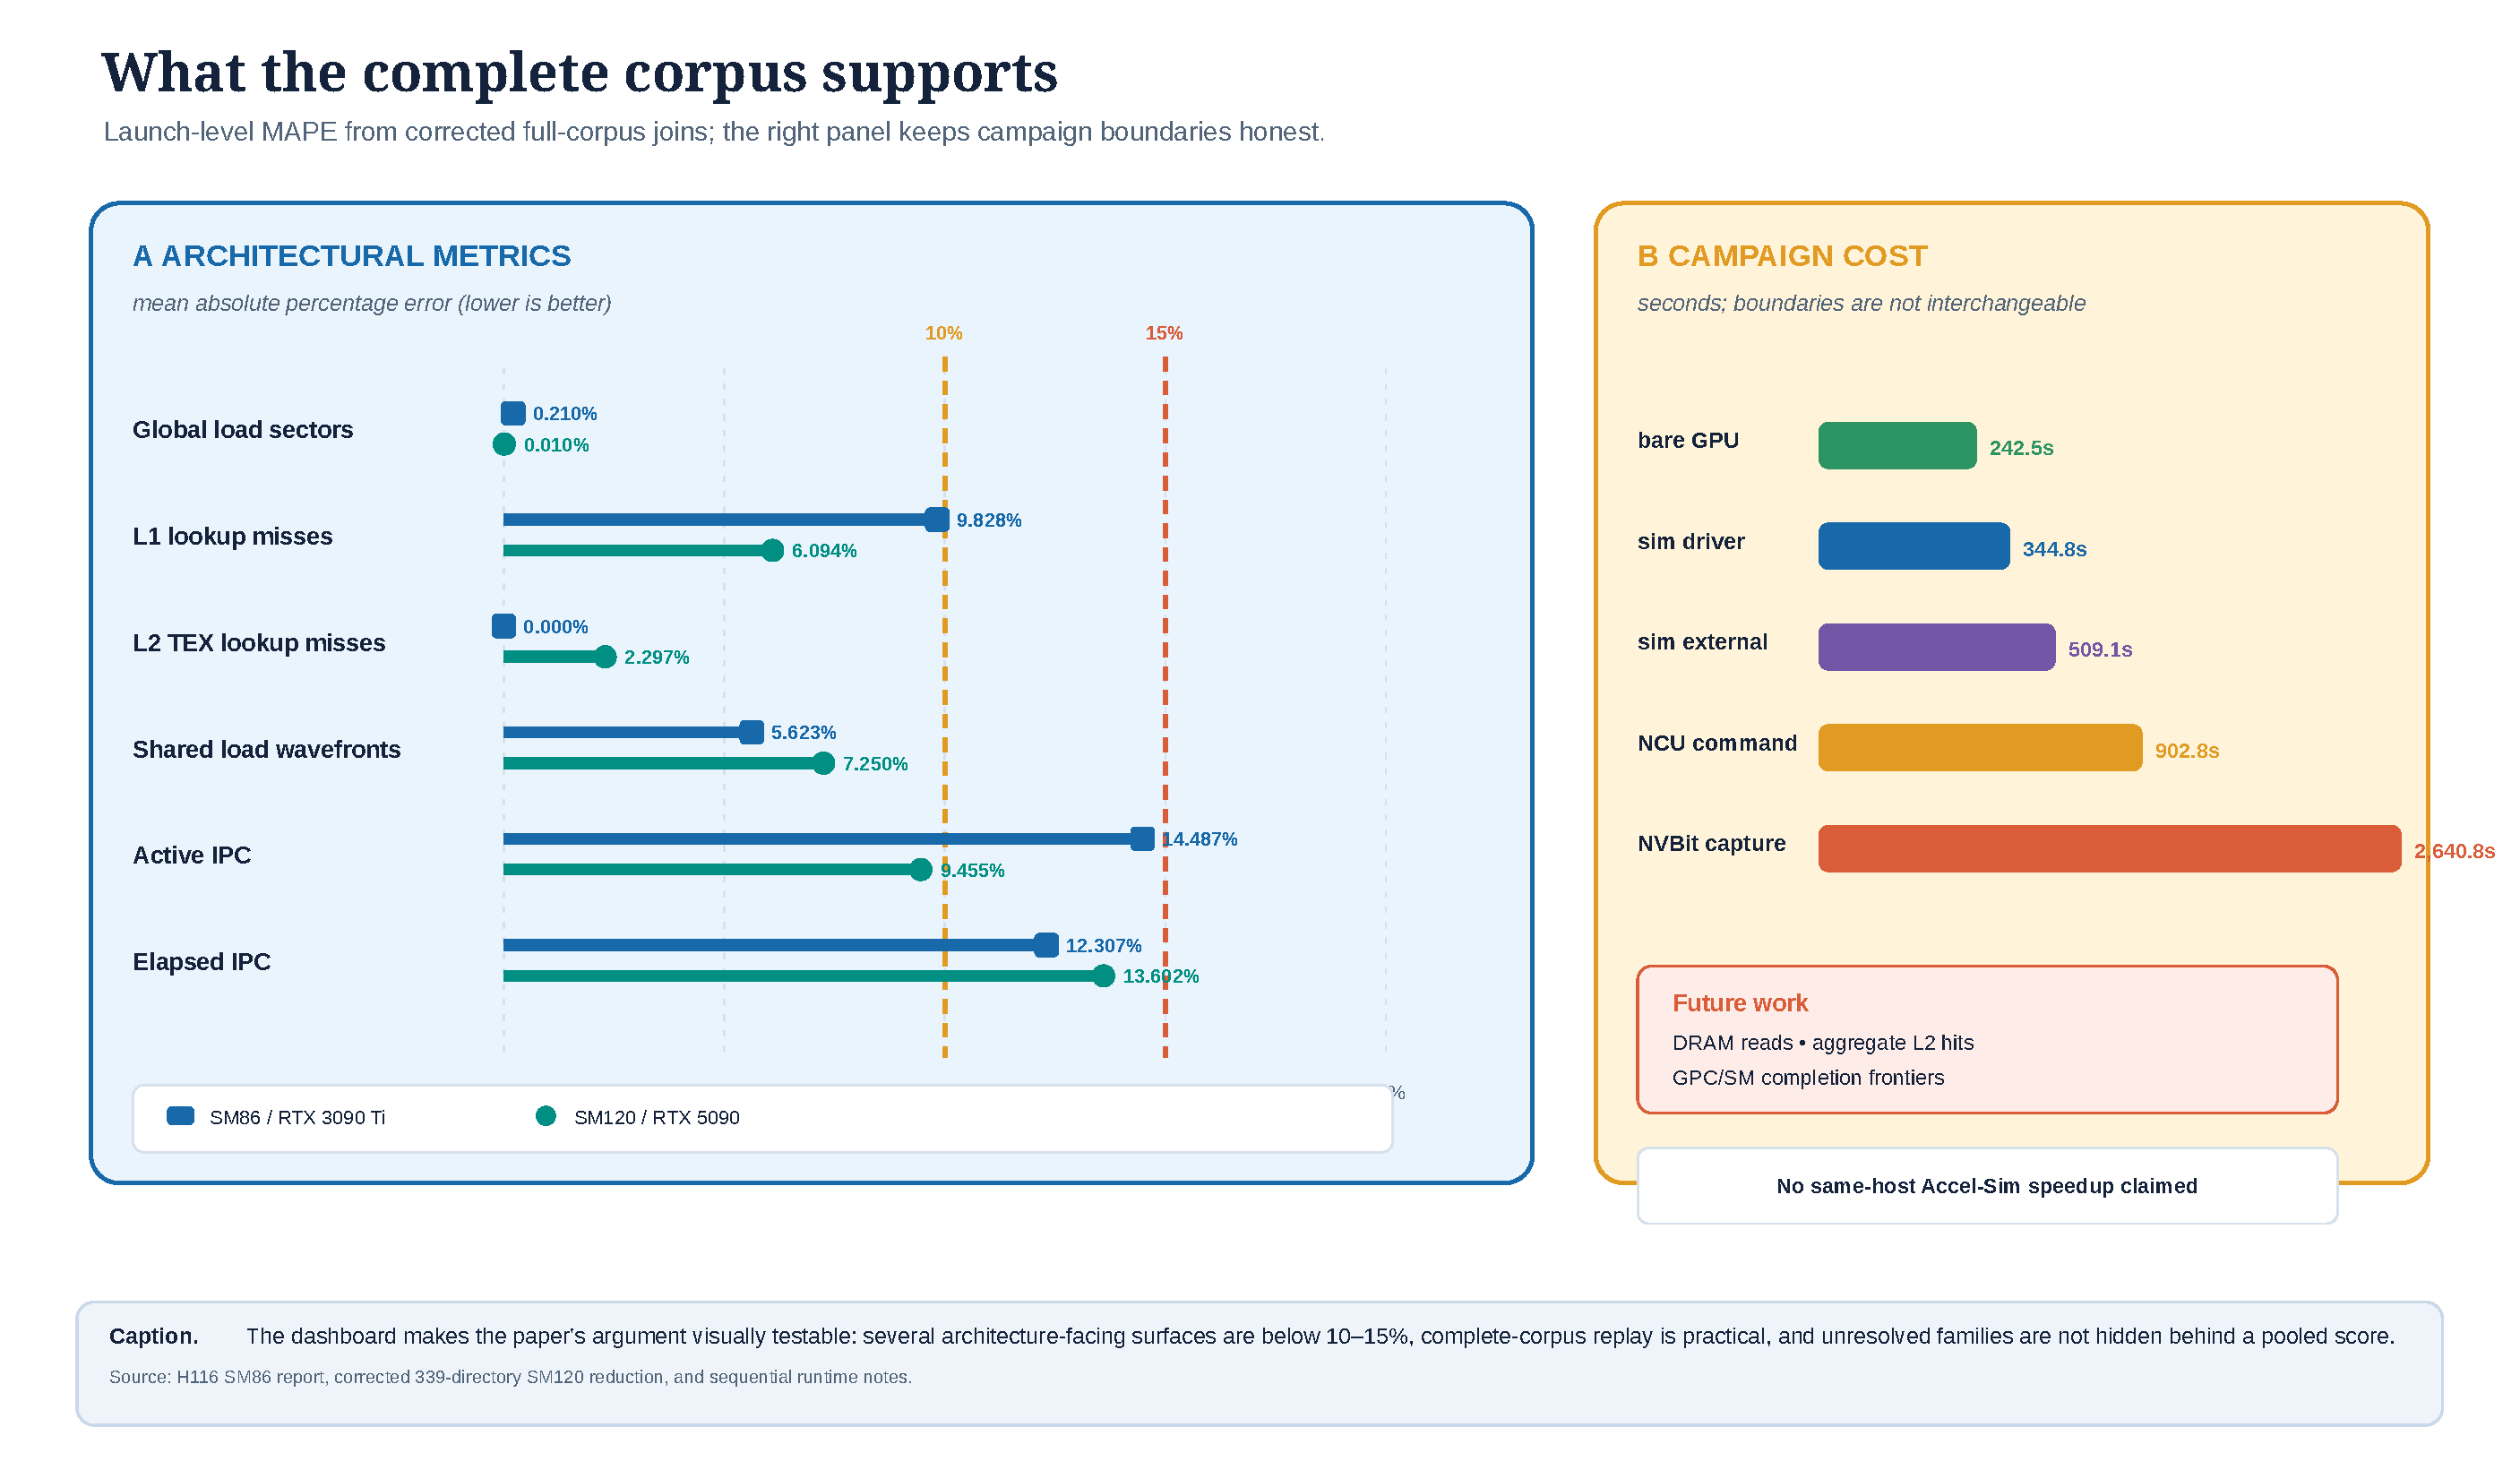
\includegraphics[width=\linewidth]{figures/results_dashboard.pdf}
  \caption{Complete-corpus results and campaign boundaries.  Panel (a) shows
  only architecture-facing metrics at or below the 15\% bar, with 10\% and
  15\% thresholds explicit.  Panel (b) distinguishes bare GPU, simulator,
  NCU, and NVBit campaign time; unresolved DRAM and completion families remain
  future work.}
  \label{fig:results-dashboard}
\end{figure}

\subsection{Replay and measurement cost}

Table~\ref{tab:runtime} keeps measurement boundaries separate.  The SM86
non-NCU workload pass is a sequential process-wall measurement on the locked
GPU.  NVBit and NCU rows are artifact-timestamp estimates for instrumented and
profiled campaign commands.  The simulator row is external runner wall time,
not just the inner event-loop sum.

\begin{table}[t]
  \centering
  \caption{Campaign wall times.  NCU and NVBit values are tool-command totals,
  not bare GPU execution time; no same-host Accel-Sim benchmark is claimed.}
  \label{tab:runtime}
  \small
  \begin{tabular}{@{}llrr@{}}
    \toprule
    Target & Phase & Workloads/roots & Total seconds\\
    \midrule
    RTX 3090 Ti & bare workload, no NCU & 286 & 242.530\\
    RTX 3090 Ti & simulator full external wall & 356 & 509.050\\
    RTX 3090 Ti & simulator driver, successful rows & 286 & 344.819\\
    RTX 3090 Ti & NVBit capture estimate & 286 & 2,640.820\\
    RTX 3090 Ti & NCU profile-command estimate & 286 & 902.797\\
    RTX 5090 & simulator full, DRAM disabled & 339 & 511.800\\
    RTX 5090 & simulator full, prototype DRAM card & 339 & 512.990\\
    RTX 5090 & NVBit capture estimate & 339 & 13,689\\
    RTX 5090 & NCU profile-command estimate & 339 & 33,159\\
    \bottomrule
  \end{tabular}
\end{table}

The SM86 simulator's successful-row driver sum is 1.42$\times$ the bare
workload process sum, while the all-root external wall includes typed controls
and replay failures.  This is strong evidence that the replay is practical for
complete-corpus iteration.  It is not a controlled claim that the simulator is
faster than Accel-Sim: the two systems were not run on the same host, with the
same trace, compiler, output, or timeout policy.  The 5090 NCU/NVBit totals are
also not directly comparable to the 3090 Ti totals because their NCU versions,
launch policies, hosts, and profile settings differ.

\section{Discussion and limitations}
\label{sec:limitations}

The high-confidence surfaces are those where the trace supplies the relevant
denominator and the model preserves sector/operation conservation.  L1 lookup
misses and L2 source lookup misses therefore meet the publication bar even
though some corresponding hit surfaces remain harder: a hit classification is
the complement of multiple client and pending-sector states, not a scalar cache
capacity law.

The current DRAM-read and completion gaps are not hidden by the table.  GCC
instruction/constant fetch ownership, maintenance and dirty writeback, exact
partition service, asynchronous engine completion, and target-dependent clock
crosswalks remain typed or future-work surfaces.  The SM120 carded bandwidth
values are a prototype hypothesis and must not be read as a locked RTX 5090
measurement.

The trace also fixes the observed dynamic path.  If a target intervention
changes an atomic order, synchronization arrival, branch, or address
calculation, fixed-trace replay answers the timing of the recorded path rather
than re-executing the program.  This is why the paper reports the trace
contract and its boundary alongside accuracy.

\section{Conclusion}
\label{sec:conclusion}

We presented an evidence-bounded trace-to-frontier replay stack for modern
NVIDIA workload traces.  Its practical novelty is the inspectable integration
of dynamic lane evidence, static SASS controls, deterministic four-partition
issue, sectored L1/L2 state, typed memory-service envelopes, separated
frontiers, and an observation-only NCU comparator.  Complete replay covers 286
SM86 and 339 SM120 capture roots, and the publication-safe metric subset meets
the declared 15\% bar with several sectors and lookup-miss surfaces below 10\%.
Sequential SM86 full replay completes in roughly nine minutes of external
runner time, while the corresponding bare workload pass is roughly four
minutes; this is a measured campaign comparison, not an unsupported
Accel-Sim speedup.  DRAM-read and completion families remain future work.  The
result is a usable, reproducible architecture-study instrument whose claims
are scoped to the evidence it actually has.

\bibliographystyle{plain}
\bibliography{references}

\end{document}
